\section{Trabalhos Relacionados}\label{sec:related}

Os trabalhos que mais se relacionam ao o aqui proposto são
aqueles que buscam transformar conjuntos de dados para
torná-los mais representativos para execução de uma
determinada tarefa.  Esses trabalhos dividem-se basicamente
em dois grupos: métodos de redução de dimensionalidade e
métodos de construção interativa de atributos. 

A seguir, na Subseção~\ref{sec:rd}, apresenta-se uma
discussão sobre os métodos de redução de dimensionalidade,
com um enfoque especial para métodos interativos. Na
Subseção~\ref{sec:tr}, apresenta-se um levantamento sobre
pesquisas em construção interativa de atributos, um tema que
não conta com uma literatura tão vasta quanto à dos métodos
de redução, mas que tem ganhado popularidade nos últimos
anos. 

\subsection{Redução de Dimensionalidade}\label{sec:rd}

O problema de se a reduzir a dimensionalidade de conjuntos
de dados pode ser descrito da seguinte forma: dado um
conjunto de dados representado por uma matriz $\textbf{X}$
composta por $n$ vetores $\textbf{x}_i~(i \in
\{1,2,...,n\})$ $m-$dimensionais, deseja-se encontrar uma
transformação $t: \textbf{X} \rightarrow \textbf{Y}$, em que
$\textbf{Y}$ é uma matriz composta por $n$ vetores
$\textbf{y}_i~(i \in \{1,2,...n\})$ de dimensionalidade $p$
($p < m$).  Normalmente $p \ll m$ e, idealmente, $p$
equivale à dimensionalidade intrínseca dos dados\footnote{A
dimensionalidade intrínseca dos dados é o conjunto
mínimo de variáveis necessárias para descrever as
propriedades dos dados~\cite{Fukunaga1990}.}, fazendo
com que $t$ mantenha em $\textbf{Y}$ o máximo das
propriedades de $\textbf{X}$ quanto for possível. 

Um dos principais objetivos da redução de dimensionalidade é
amenizar os efeitos da maldição da
dimensionalidade\footnote{A maldição da dimensionalidade foi
    um termo introduzido por \citet{Bellman1961} para se
    referir aos problemas que surgem ao lidar com conjuntos
    de dados com um elevado número de dimensões (centenas ou
    milhares). Sua maior implicação é a falta de
separabilidade entre elementos que se encontram em um espaço
de alta dimensão~\cite{Kouiroukidis2011}.} e com isso fazer
com que os métodos que operam sobre os dados tenham uma
melhor eficiência e um menor custo
computacional~\cite{Maaten2009}.  
Uma segunda utilidade para os métodos de redução de
dimensionalidade é viabilizar a construção de representações
visuais de dados multidimensionais, permitindo que sejam
mapeados em um espaço bidimensional (tela computador).
Representações visuais têm sido fundamentais para análises
exploratórias de dados, principalmente em investigações
iniciais, onde não
se conhece as propriedades dos dados~\cite{Kaski2011}. 

A literatura em redução de dimensionalidade é extensa e os
métodos desenvolvidos apresentam grande diversidade em
relação a aspectos matemáticos e computacionais. Buscando
uma melhor contextualização, discute-se aqui apenas
trabalhos que buscam de alguma forma utilizar representações
visuais para a execução desta tarefa.

Métodos visuais que permitem a interação do usuário ganharam
grande popularidade nos últimos anos~\cite{State2012}.
Grande parte deste sucesso pode ser atribuído ao uso efetivo
da capacidade preemptiva da visão humana. Foi demonstrado
que quando os dados são representados por alguma forma
gráfica, o ser humano é capaz de detectar e reconhecer
padrões facilmente e rapidamente~\cite{Healey1995}, mesmo em
grandes conjuntos de dados~\cite{Fodor2002}. Mas utilizar a
capacidade preemptiva de visão humana não é a única vantagem
dos métodos visuais. Permitir que o usuário participe
ativamente nos processos e na geração dos resultados é um
dos grandes benefícios desses métodos. Deste
modo, a seguir serão apresentados os trabalhos desta 
vertente que buscam executar redução de dimensionalidade de
forma interativa. Trabalhos que não somente fazem uso da
capacidade perceptiva humana, mas que também permitem
que o usuário participe ativamente na geração dos resultados
com o seu conhecimento sobre o domínio.

\subsubsection{Matrizes de Correlação}\label{sss:cormat}

Uma das maneiras mais utilizadas para se inspecionar
relações entre dimensões são as matrizes de
correlação~\cite{Friendly2002}. O objetivo desse modelo
visual não é propriamente reduzir a dimensionalidade do
conjunto de dados, mas sim ajudar o usuário a encontrar
subconjuntos de atributos com características de interesse.

Devido à sua simplicidade, esse tipo de representação têm
sido adotada por diversos métodos visuais que viabilizam a
investigação de atributos de conjuntos de
dados\citet{Friendly2002,Guo2003,MacEachren2003,
RBF2004,May2011ss,Johansson2009,Ingram2010,May2011}. Eles
diferem na maneira de como é construída a matriz de
correlação e de quais recursos são disponibilizados para o
usuário interagir com os subconjuntos de dimensões. Um
problema geral desses trabalhos é que certas análises podem
exigir demasiado esforço do usuário devido à necessidade de
se explorar individualmente cada dimensão ou avaliar
par-a-par as relações entre atributos. Com a ocorrência de
dependências não lineares este problema torna-se ainda maior
e o usuário pode se perder em suas análises e não extrair
novos conhecimentos dos resultados. 

A seguir apresenta-se alternativas às matrizes de correlação
para se apresentar medidas de correlação. Essas abordagens
fornecem mecanismos mais diretos para se reduzir a
dimensionalidade dos conjuntos de dados. 

\subsubsection{Hierarquias de Dimensões}

Em busca de construir espaços de baixa dimensionalidade mais
intuitivamente do que pelo uso de métodos automáticos,
\citet{Yang2003} desenvolveram o método de redução de
dimensionalidade chamado VHDR (\emph{Visual Hierarchical
Dimensions Reduction}). O funcionamento deste método é
ilustrado pela Figura~\ref{fig:vhdr1}. Inicialmente (1),
constrói-se uma organização hierárquica dos atributos com
base na similaridade entre as dimensões. Em seguida (2), o
usuário define os níveis da hierarquia que devem ser
considerados pela última etapa do processo. Finalmente (3), o
usuário por meio de um método automático ou de seu
conhecimento sobre os dados, escolhe dimensões
representativas para os níveis definidos, reduzindo assim a
dimensionalidade dos dados. 

\begin{figure}[h!]
  \centering
  \begin{subfigure}[b]{0.35\textwidth}
    \centering
    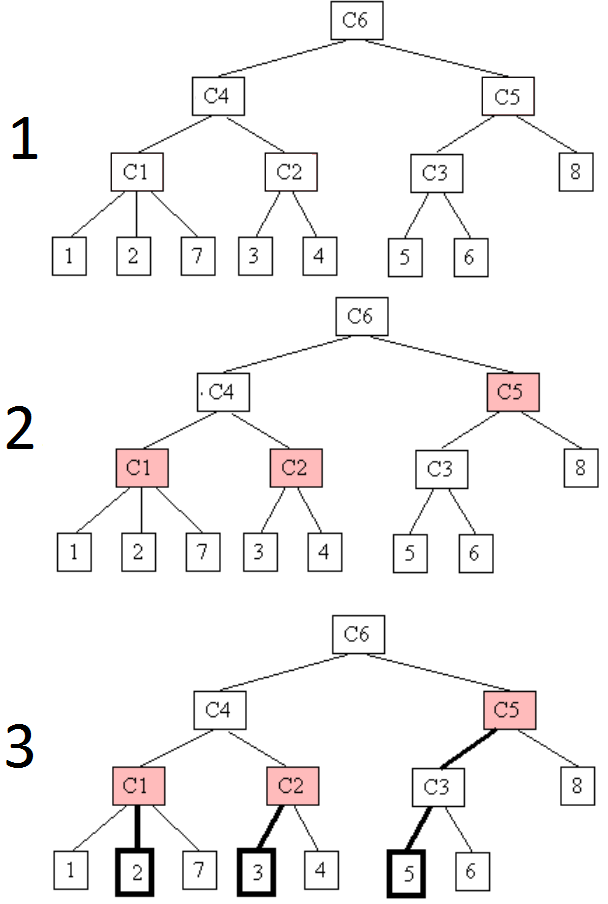
\includegraphics[width=\textwidth]{images/vhdr1.png}
    \caption{}
    \label{fig:vhdr1}
  \end{subfigure}%
  \hspace{1cm} %add desired spacing between images, e. g. ~, \quad, \qquad etc.
  \begin{subfigure}[b]{0.5\textwidth}
    \centering
    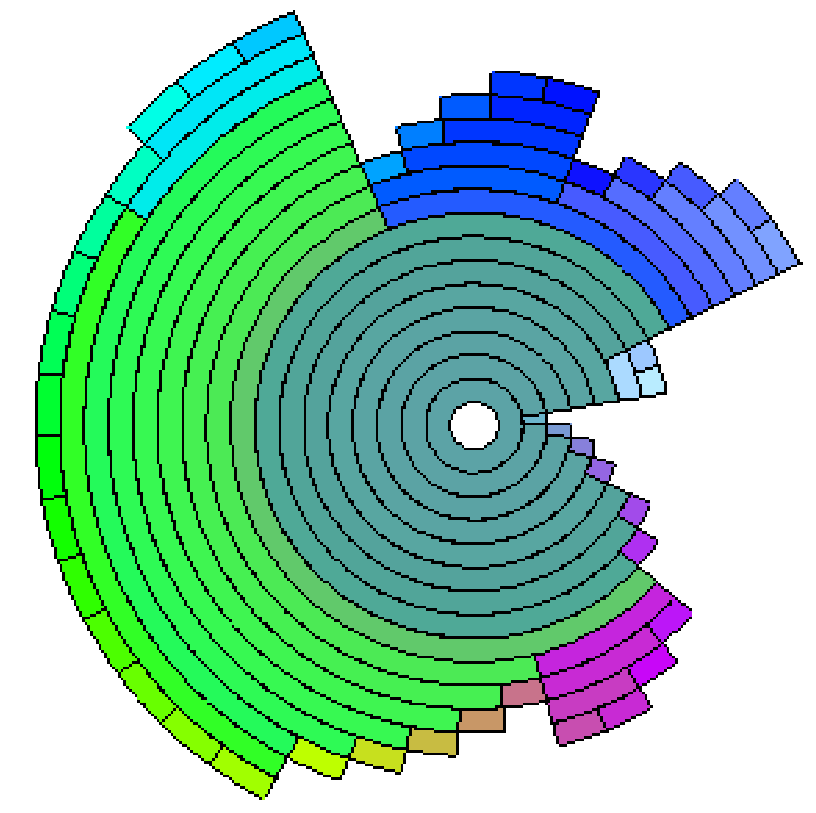
\includegraphics[width=\textwidth]{images/vhdr2.png}
    \caption{}
    \label{fig:vhdr2}
  \end{subfigure} \caption[VHDR: Visual Hierarchical
  Dimension Reduction]{(a) Ilustração do funcionamento do
  VHDR. (b) Exemplo da representação gráfica adotada pelos
  autores do VHDR. Ambas imagens extraídas de
  \cite{Yang2003}.}
\end{figure}

O processo de construção da hierarquia é muito semelhante
aos algoritmos de agrupamento hierárquico. A distinção é que
agrupa-se atributos semelhantes, ao invés de itens. Deste
modo, qualquer método de agrupamento pode ser aplicado,
exigindo-se apenas que o agrupamento resulte em uma
estrutura hierárquica, no caso uma árvore, onde cada
dimensão seja representada por um nó folha da árvore. 

A representação gráfica utilizada no VHDR é a
\emph{InterRing}~\cite{Yang2002} e pode
ser observada na Figura~\ref{fig:vhdr2}. O nó raiz da árvore
é representado pelo círculo mais interno e os nós folhas
pelos elementos posicionados na borda. As cores são
utilizadas para destacar grupos de dimensões com
características em comum. 

Os autores do VHDR desenvolveram uma extensão chamada DOSFA
(\emph{Dimension Ordering Spacing and Filtering
Approach})~\cite{DOSFA} que apresenta outras abordagens para
investigar os atributos de um conjunto de dados. Mais
especificamente, eles propõem ferramentas para ordenação,
espaçamento e filtragem de atributos. As duas primeiras,
ordenação e espaçamento, não estão diretamente relacionadas
com redução de dimensionalidade. Já a filtragem de atributos
é análoga aos métodos de seleção de características. Este
mecanismo consiste em remover dimensões pouco
representativas ou redundantes, de modo que se certas
dimensões apresentam alta similaridade entre si, então
apenas uma delas é mantida, ou se certas dimensões
apresentam pouca relevância, então são descartadas. A grande
complexidade do processo de filtragem esta no modo como se
define a redundância e a importância entre as dimensões. Um
método semelhante para filtragem de atributos irrelevantes
foi proposto por \citet{Artero2006}.

Tanto o VHDR quanto o DOSFA tratam todo o conjunto de dados
de maneira uniforme. No entanto, podem existir subconjuntos
nos dados com diferentes características que devem ser
analisados separadamente~\cite{May2011}. Uma maneira de
contornar este problema seria apresentar os itens
simultaneamente com a representação das dimensões, assim o
usuário poderia detectar grupos não somente nas dimensões
mais também nos itens. Criar tal representação é o objetivo
dos trabalhos discutidos a seguir.

\subsubsection{Mapeamento de Elementos no Plano}

Abordando justamente o problema de se apresentar itens
simultaneamente com as dimensões de um conjunto de dados,
\citet{Yang2004} desenvolveram a ferramenta VaR (\emph{Value and
Relation}). A abordagem une os conceitos de MDS e glifos para
representar as dependências entre as dimensões de uma base
de dados. 

\begin{figure}[h!]
  \centering
  \begin{subfigure}[b]{0.5\textwidth}
    \centering
    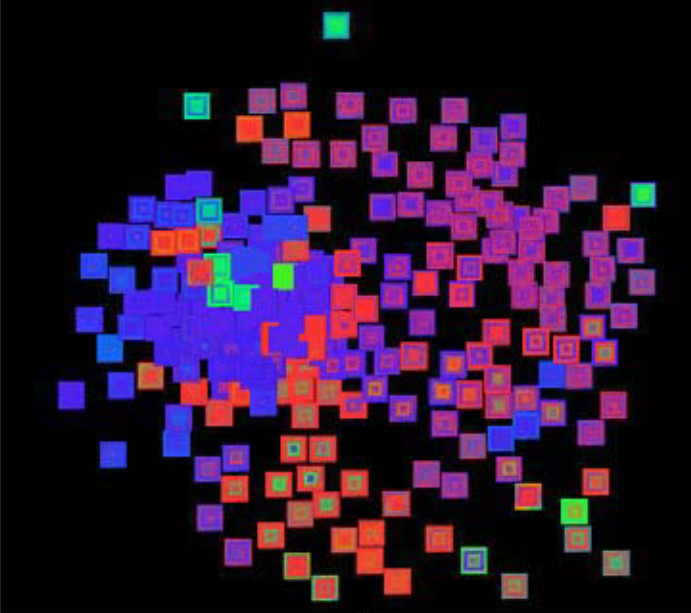
\includegraphics[width=\textwidth]{images/var1.png}
    \caption{}
    \label{fig:var1}
  \end{subfigure}%
  ~ %add desired spacing between images, e. g. ~, \quad, \qquad etc.
  \begin{subfigure}[b]{0.475\textwidth}
    \centering
    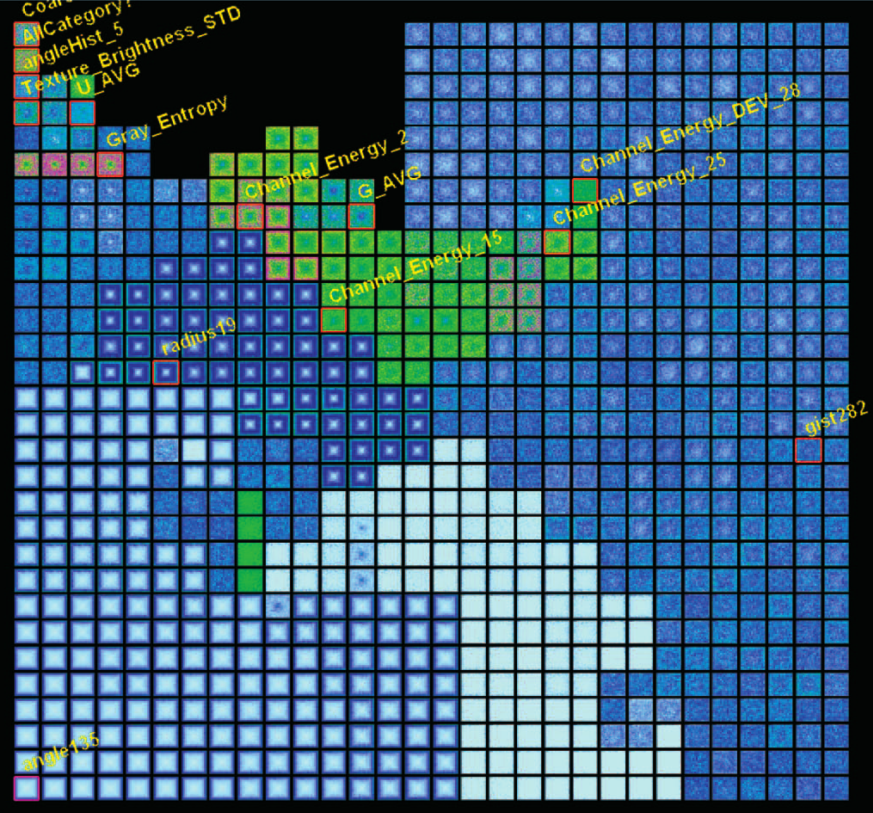
\includegraphics[width=\textwidth]{images/var2.png}
    \caption{}
    \label{fig:var2}
  \end{subfigure}
  \caption[VaR: Value and Relation]
      {(a) Exemplo da ferramenta VaR. Imagem extraída de
      \cite{Yang2004}. (b) Exemplo da representação
  alternativa proposta como extensão da ferramenta VaR.
  Imagem extraída  de \cite{Yang2007}.}
\end{figure}

Na representação visual da ferramenta VaR, cada dimensão é
representada por um glifo e seus posicionamentos refletem a
similaridade entre as dimensões, de modo que glifos que se
encontram próximos indicam atributos que apresentam alguma
relação entre si. Como mostra a Figura~\ref{fig:var1}, de
acordo com o posicionamento dos glifos no plano o usuário
pode compreender como as dimensões se relacionam entre si. O
usuário é capaz de construir espaços dimensionais reduzidos
que conservam certas características dos dados por meio de
seleções manuais sobre os dados ou pelo uso de um método automático.
Este método automático parte de uma dimensão de referência e
de um limiar definido pelo usuário e retorna as dimensões
mais semelhantes à esta referência.

Observando a Figura~\ref{fig:var1} é possível notar que o
uso de glifos faz com que ocorram sobreposições, pois cada
glifo requer um espaço relativamente grande para que seja
observado adequadamente.  As sobreposições dificultam as
análises de regiões de interesse e podem fazer com que o
usuário alcance conclusões inválidas, devido a oclusão de
algum elemento importante.  

Buscando tratar o problema de sobreposição de elementos,
\citet{Yang2007} desenvolveram a extensão ilustrada na
Figura~\ref{fig:var2}, onde apresentaram alternativas para o
mapeamento dos glifos no plano. No entanto, a alternativa
proposta estabelece uma distância fixa entre os elementos,
consequentemente perde-se a informação de quanto duas
dimensões são similares entre si. Assim, o resultado obtido
pela versão original transmite melhor os relacionamentos entre
as dimensões do que a abordagem proposta na extensão. 

Apesar da ferramenta VaR apresentar informações sobre itens
e dimensões simultaneamente, não é permitido ao usuário
interagir com os itens. Consequentemente, esta abordagem
sofre das mesmas limitações das ferramentas apresentadas
anteriormente, ou seja, não é capaz de lidar com  
características locais em subconjuntos dos dados. Um outro
aspecto importante que os próprios autores mencionam em
relação ao uso de glifos é que os usuários têm dificuldade
em comparar glifos que se encontram afastados entre si. 

O trabalho proposto por \citet{Turkay2011}, \emph{Brushing
Dimensions} (BD), cobre esse limitação da ferramenta VaR,
pois permite aos usuários interagir tanto com as dimensões
dos conjunto de dados quanto com os itens. Semelhantemente à
ferramenta VaR, as representações visuais do BD são baseadas
em mapeamentos de elementos no plano. As representações dos
itens são construídas com base em métodos automáticos, como
PCA, e as das dimensões por medidas estatísticas, como média
e variância. Este modo de posicionamento das dimensões é uma
das limitações da ferramenta, pois ao desconsiderar medidas
par-a-par, como correlação, a visualização não apresentará
dependências entre os atributos. O principal mecanismo de
interação da ferramenta BD é a seleção que se reflete em
outras visões e permite que se visualize, por exemplo,
variações na importância de um atributo em diferentes
subconjuntos dos dados. Uma das limitações de ambos os
métodos, VaR e BD, é não permitir que o usuário construa
novas dimensões com base nas originais ou
com base no seu conhecimento.

Uma questão inerente de se mapear elementos de um espaço de
alta dimensionalidade em um plano, sejam os elementos itens
ou dimensões, é que não há garantias de que o mapeamento
seja válido. Em casos onde a dimensionalidade intrínseca dos
dados for maior do que ao do espaço alvo, então poderá haver
sobreposição de elementos sem necessariamente significar que
os elementos sobrepostos sejam realmente semelhantes. Ambos
VaR e BD não atentam para esta questão, mas
\citet{Ingram2010} desenvolveram a ferramenta
\emph{DimStiller} (DS) buscando construir mapeamentos de
dados multidimensionais levando em consideração este
problema. 

Um outro aspecto importante da redução de dimensionalidade,
que muitas vezes não é levado em consideração, é que
dependendo do método adotado, diferentes características dos
dados podem ser mantidas e outras perdidas. Este problema é
abordado no trabalho de \citet{Johansson2009}, onde por meio
de gráficos de perda de informação para diferentes medidas,
o usuário pode entender quais características dos seus dados
são mantidas e perdidas ao longo do processo de redução. 

O trabalho de \citet{Johansson2009}, assim como o
\emph{DimStiller}, pode ser dito consciente de incerteza.
Isso, pois se preocupam em apresentar aos usuários os fatores que
podem resultar em interpretações ambíguas dos resultados e
na perda de possíveis informações de interesse. 
Tal preocupação não é presente em muitas das ferramentas de
visualização atuais, mas tem se tornado cada vez mais uma
exigência~\cite{Dill2012}.

As ferramentas de redução de dimensionalidade não são
restritas a totalmente automáticas ou integralmente
interativas. Abordagens mistas podem ser adotadas, como é o
caso dos trabalhos discutidos a seguir.

\subsubsection{Visualização de Métodos Automáticos}

Existem métodos que não fazem uso de representações
visuais para realizar a redução de dimensionalidade em si,
mas sim para tornar os métodos automáticos mais
compreensivos. Eles buscam incluir a participação do usuário
nesse processo para tornar essas ``caixas pretas'' mais
intuitivas. 

A ferramenta iPCA~\cite{Jeong2009}, por exemplo, provê meios
para o usuário manipular os parâmetros da técnica PCA e,
assim, ser capaz de entender mais facilmente as
transformações realizadas sobre os dados. Similarmente,
\citet{Williams2004} permitem que o usuário guie o processo
de redução de dimensionalidade a partir de métodos MDS ao
escolher regiões de interesse para se concentrar os esforços
computacionais.  Neste mesmo sentido, \citet{Schreck2008}
desenvolveram uma ferramenta que permite ao usuário
monitorar visualmente os recursos computacionais utilizados
pelo método SOM e definir interativamente os parâmetros para
sua execução.

Dentro do contexto de seleção de características, o trabalho
de \citet{Dy2000} busca tornar este processo mais interativo.
Possibilitando ao usuário escolher grupos de itens para
análises mais detalhadas e fornecendo mecanismos interativos
para adição e remoção de atributos em cada etapa dos métodos
de seleção. O trabalho de \citet{Brandoli2010} apresenta um
objetivo similar, porém com um enfoque em auxiliar o
usuário a definir os parâmetros dos métodos de seleção de
características.

Os trabalhos propostos por \citet{Zhang2006}, \citet{Choo2010}
e \citet{Paiva2012} são abordagens que buscam tornar o
processo de redução de dimensionalidade mais intuitivo no
contexto de classificação de dados. Nesses métodos a redução
de dimensionalidade reflete diretamente na qualidade das
classificações. 

Um problema das ferramentas que criam visualizações de métodos
automáticos é a necessidade do usuário ter um certo
conhecimento sobre o método por trás da visualização. Por
exemplo, no caso da ferramenta iPCA, o usuário pode ver
pouca utilidade na visualização da janela B apresentada na
Figura~\ref{fig:ipca} se não souber o que significa um
componente principal. Para pesquisadores da área pode ser
até pressuposto que o usuário tenha este tipo de
conhecimento, no entanto, se o objetivo for criar uma
ferramenta para o público em geral, então tal suposição pode
restringir o seu uso.

\subsection{Construção Interativa de Atributos}\label{sec:tr}

Os métodos de redução de dimensionalidade realizam
transformações sobre os dados, porém, mesmo as ferramentas
interativas de redução não permitem que o usuário modifique
os atributos livremente. A construção interativa de
atributos significa mais do que permitir que o usuário guie
as transformações sobre os dados, trata-se de permitir que o
usuário agregue seu conhecimento sobre os dados. 

Esse tipo de abordagem ainda não conta com uma literatura
tão vasta quanto a dos métodos de redução de
dimensionalidade. Sendo que a principal contribuição é a
ferramenta proposta por \citet{Gladys2013} que possibilita ao
usuário modificar os atributos de um conjunto de dados com
base na manipulação sobre amostras dos itens. Os autores
fazem uso de mapeamento de elementos no plano para permitir
interações intuitivas sobre os dados. 

A Figura~\ref{fig:ud} apresenta  o funcionamento dessa
ferramenta. Inicialmente, o usuário manipula uma amostra dos
dados buscando  agrupar elementos que considera similares.
Em seguida, as manipulações realizadas sobre a amostra são
refletidas para o conjunto de dados original, fazendo com
que este reflita a opinião do usuário em relação ao critério
de similaridade entre os elementos. Este processo pode ser
repetido até que se atinja o resultado esperado. Observa-se
que para este exemplo a transformação do espaço foi bem
sucedida, pois foram reveladas estruturas que até então não
eram identificáveis.

\begin{figure}[h!]
    \centering
    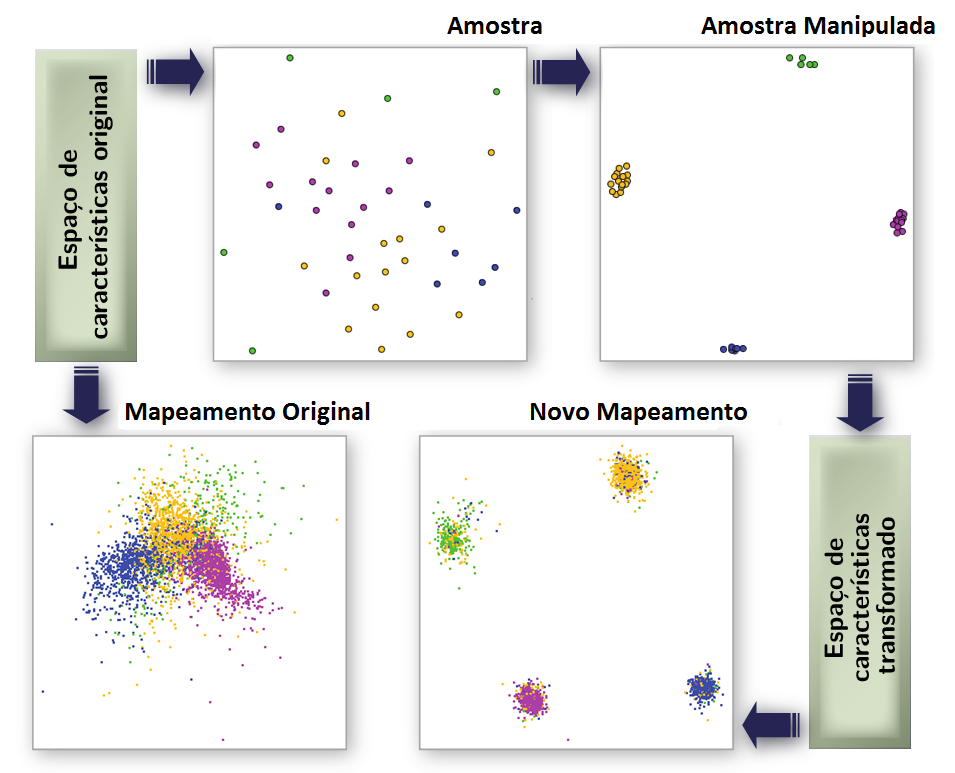
\includegraphics[width=10cm]{images/ud.png}
    \caption{Ferramenta desenvolvida por \cite{Gladys2013}.}
    \label{fig:ud}
\end{figure}

Por se tratar de uma abordagem pioneira, essa ferramenta
possui diversas limitações. Por exemplo, a forma como a
amostragem é realizada não garante de que elementos de cada
estrutura presente nos dados são escolhidos.
Consequentemente, exige-se mais iterações do usuário 
para que seu conhecimento seja agregado aos dados. Portanto,
existem inúmeras possibilidades de trabalhos futuros para
pesquisas em construção interativa de atributos.

\subsection{Considerações Finais}

Nesta seção foram apresentados ferramentas que viabilizam a
modificação interativa de conjuntos de dados de modo a
torná-los mais representativos para a compreensão do
fenômeno em estudo.  Nas discussões foram levantadas uma
série de limitações dos trabalhos do atual estado da arte.
Tal levantamento foi levado em consideração para a escrita
da proposta deste projeto de trabalho de mestrado, a qual é
apresentada na seção a seguir.
